\documentclass[reprint,nofootinbib,...]{revtex4-1} 
%\documentclass[draft,nofootinbib,...]{revtex4-1} 
\usepackage{amsmath}%
\usepackage{amsthm,amssymb}
\usepackage{graphicx}
\usepackage{epstopdf}
\usepackage{xcolor}
\usepackage{algcompatible}
\usepackage[size=small]{caption}
\usepackage{etoolbox}
\usepackage{booktabs}
\usepackage{multirow}
\usepackage[utf8]{inputenc}
\usepackage[colorinlistoftodos]{todonotes}

\usepackage[hyperfootnotes=true]{hyperref}
\hypersetup{
 colorlinks=true,
 citecolor=blue,
 linkcolor=blue,
 urlcolor=blue}
 
 \DeclareMathOperator{\sign}{sign}
 \DeclareMathOperator*{\argmin}{argmin}
 \DeclareMathOperator*{\E}{\mathbb{E}}
 
% some placeholders for various parameters of the network, dataset, experiments, etc
\newcommand{\nconst}{64}       % number of jet constituents

\newcommand{\JetPtMin}{300}    % minimum jet pT [GeV]
\newcommand{\JetMassMin}{50}   % minimum jet mass [GeV]

\newcommand{\HLLayers}{3}
\newcommand{\HLUnits}{384}
\newcommand{\HLAuc}{0.79}

\newcommand{\PfnPhiLayers}{4}
\newcommand{\PfnFLayers}{4}
\newcommand{\PfnUnits}{256}
\newcommand{\PfnAuc}{0.87}

\newcommand{\ptcut}{1.3}           % leading jet pT cut
\newcommand{\nlayerCLS}{3}     % number of layers in the target classifier
\newcommand{\nunitsCLS}{256} % number of units per layer
\newcommand{\ntrain}{145k}       % number of training samples
\newcommand{\nval}{26k}            % number of validation samples

\newcommand{\aucCLS}{0.88}    % validation AUC of benchmark classifier

\newcommand{\epsilsonpt}{0.99} % Epsilon values for pt/eta/phi in FGSM attack
\newcommand{\epsiloneta}{0.99}
\newcommand{\epsilonphi}{0.99}

%adversarial network parameters
\newcommand{\nlayerADV}{3}
\newcommand{\nunitsADV}{512}

% convenience defs
\newcommand{\pt}{p_\mathrm{T}} % needs mathmode

%%% ----------------------------------------------------------------------
\begin{document}

%Title of paper
\title{AI Safety for High Energy Physics}

\author{Benjamin Nachman}
\email{bpnachman@lbl.gov}

\affiliation{Physics Division, Lawrence Berkeley National Laboratory, Berkeley, CA 94720, USA}

\author{Chase Shimmin}
\email{chase.shimmin@yale.edu}

\affiliation{Department of Physics, Yale University, New Haven, CT 06511, USA}


\begin{abstract}

The field of high-energy physics (HEP), along with many scientific disciplines, is currently experiencing a dramatic influx of new methodologies powered by modern machine learning techniques.
Over the last few years, a growing body of HEP literature has focused on identifying promising applications of deep learning in particular, and more recently these techniques are starting to be realized in an increasing number of experimental measurements.
%% CS: Not sure if it's a good idea to have references in the abstract? Also, maybe we shouldn't jump right in with jargon like "low-level featuers".
%Since the first application of deep learning on `low-level' features for classification in high-energy physics (HEP)~\cite{Baldi:2014kfa}, there has been a rapidly expanding literature on the adaptation of industrial deep learning techniques as well as the development of novel methods.
The overall conclusion from this impressive and extensive set of studies is that rarer and more complex signatures can be identified with the new set of powerful tools from deep learning.  However, there is an unstudied systematic risk associated with combining the traditional HEP workflow and deep learning with high-dimensional data.
In particular, calibrating and validating the response of deep neural networks is in general not experimentally feasible, and therefore current methods may be biased in ways that are not covered by current uncertainty estimates.
By borrowing ideas from AI safety, we illustrate these potential issues and propose a method to bound the size of unaccounted for uncertainty.
In addition to providing a pragmatic diagnostic, this work will hopefully begin a dialogue within the community about the robust application of deep learning to experimental measurements and searches.
\end{abstract}

\date{\today}
\maketitle

%%%%%%%%%%%%%%%%%%%%%%%%%%%%%


\section{Introduction}
\label{sec:intro}
%%% Note: having a hard time striking a balance between explaining how we do analysis at the LHC, so that other fields can understand the problem,
%%% vs, keeping this short and generic enough to underscore how it applies other fields.
Experiments in collider-based high-energy physics (HEP) rely critically on detailed simulations which model length scales from sub-nuclear reactions all the way to macroscopic detector-length scales in order to connect fundamental theories to experimentally-observable quantities.
Typical experiments, such as measurements of physical constants or searches for new particle species, are designed using blinded methodology, and depend on these calibrated simulations to predict the relative rates of background and signal events.
These predictions are in turn used to define the statistical significance and/or confidence intervals of the results observed after unblinding.
While the simulations involved in this process highly sophisticated, they are only an approximation to reality and therefore systematic mismodelling must be accounted for by calibrating to data, when possible, and by assessing systematic errors.

Traditionally, partitions of the data known as \textit{signal} and \textit{control regions} are defined by applying selective criteria on physical observables, in order to isolate regions of the data that are expected to be sensitive to the phenomena of interest from well-understood phenomena.
It is then possible to validate and/or calibrate the simulated background predictions against data observed in the signal-free region without biasing the blinded analysis.
However, it is often the case that several different observables, perhaps following some complicated relationship, are useful for defining such regions of the data.
A typical application of machine learning in HEP is to automate the construction of signal and control regions by reformulating the task as an optimization problem; for example, a binary classifier may be trained on simulations to label observed events as signal-like or background-like.
While this has been done for years using ``shallow'' classifiers such as Boosted Decision Trees, the success of these methods have generally depended strongly on the choice of features input to the classifier, incurring a significant amount of effort towards ``feature engineering'' to identify useful \textit{high-level} observables.

%In the traditional paradigm, a set of discriminating observables are used to isolate a region $s$ of phase space called the \textit{signal region}, where the expected rate of a hypothetical signal is large relative to the SM background.
%The sensitivity of this approach is generally related to the relative rates of the signal and background, as well as the precision with which the background may be estimated.
%In order to constrain the latter, a separate region $c$ of phase space is defined, where contributes from new physics are expected to be negligible, providing a pure sample of SM background processes.
%In this \textit{control region}, the simulation is adjusted to match the observed data.  For example, this may be done by scaling an unknown normalization, or by constraining nuisance parameters of the simulation model.  The adjust simulation is then used to make a prediction for the background rate in the signal region by extrapolation. 


%Signal and control regions are defined by applying selective criteria on physical observables, such as particle momenta or topological structure of an event.  It is often the case that many observables, perhaps in some complicated relationship, are useful for isolating signal and background processes.
%A typical application of machine learning in HEP is to automate the construction of signal and control regions by formulating the task as an optimization problem.  For example, a binary classifier may be trained on simulation to distinguish signal events from background events and then $s$ and $c$ could correspond to different regions of the classifier output.  While this has been done for years\footnote{See for instance Ref.~\cite{Hocker:2007ht} and the papers that cite it.} using ``shallow'' classifiers, the success of these methods have generally been very sensitive to the exact observable features selected as input to the classifier, incurring a significant amount of effort towards ``feature engineering'' to identify useful \textit{high-level} observables.

With the more recent introduction of deep learning methods, it has become possible to construct increasingly elaborate classification models using higher-dimensionality input features.
Perhaps surprisingly, it has been shown\footnote{There are now too many examples to cite them all here.  References~\cite{Larkoski:2017jix,Radovic:2018dip,Guest:2018yhq} are recent reviews of deep learning in HEP and References~\cite{Baldi:2014kfa,deOliveira:2015xxd,Baldi:2016fql,Guest:2016iqz} were the earliest applications of deep learning to collider-based HEP classification problems.} that when provided with high-dimensional \textit{low-level} (HDLL) features (\textit{i.e.} observables that are minimally processed using physical intuition), deep neural networks are able to automatically learn to exceed the performance of networks trained on physically-motivated high-level features.

%Deep learning offers a new set of tools in HEP for seeking out new particles using high-dimensional, low-level information~\cite{Baldi:2014kfa,Larkoski:2017jix,Radovic:2018dip,Guest:2018yhq}.
%A growing number of searches at the Large Hadron Collider are using deep learning methods to construct $m$.
%The control region method is the baseline approach for estimating the SM background in the nascent deep learning era.

Increasingly, experimentalists at the Large Hadron Collider (LHC) and elsewhere are taking this message seriously.
While the first analysis-level deep learning results from the LHC are only starting to become public (see e.g.~\cite{Aad:2019yxi,ATLAS-CONF-2019-017,CMS-PAS-SUS-19-009}), analysis-non-specific deep learning models have been used for a few years, notably with early successful applications in flavor tagging~\cite{CMS-DP-2017-005,ATL-PHYS-PUB-2017-003}.
In addition, there is a plethora of experimental and phenomenological studies for additional methods which will likely be realized as part of physics analyses in the near future.
This includes proposals to use the lowest-level inputs available to from the detector, reaching input feature dimensionalities of $\mathcal{O}(10^5)$~\cite{Andrews:2018nwy,Andrews:2019faz} and beyond.
% @Ben: why is the following removed? Maybe it can be rephrased but I think it's worth making the case that the issue at hand is not isolated to our specific (sub)field.
%This trend is also seen in related fields such as neutrino physics, where various TPC detector experiments are moving towards deep learning on very low-level data to replace conventional event reconstruction methods~\cite{Acciarri:2016ryt,Delaquis:2018zqi}.



A potential problem with this approach arises when combining deep learning on HDLL features with the conventional simulation-based analysis paradigm.  In the traditional approach, uncertainties on the extrapolation between the control region and the signal region rely on simulation variations that can be validated on a small number of one-dimensional physically-motivated features.  Correlated uncertainties covering the full HDLL feature space are often not known or experimentally infeasible~\cite{Nachman:2019dol}.
Moreover, low-dimensional validation may be insufficient: recent developments in the area of Artificial Intelligence (AI) safety have demonstrated that when neural networks operate on high-dimensional input spaces, classification performance of neural networks can be arbitrarily degraded by applying subtle variations to the input features~\cite{Szegedy14intriguingproperties,DBLP:journals/corr/GoodfellowSS14}.

%This work uses methods from AI safety to diagnose the sensitivity of the current methodology to under-constrained feature spaces.
%In particular, a common high-dimensional classification problem from jet physics is used to illustrate the sensitivity to small perturbations in measured particle properties and also to devise a sensitivity diagnostic with a directed adversarial attack.
%Certainly nature is not evil, but without any good estimate of high dimensional correlated uncertainty, this bound can be used to demonstrate robustness. 

To illustrate this challenge, we implement an adversarial attack that demonstrates small perturbations in detector-level measurements can have drastic effects on the performance of a neural network trained to identify signal-like events.
This adversarial procedure can be conceptualized as a sort of \textit{demon}~\cite{TheLordKelvin} which intercedes between a physical process and the observation of that process, in such a way as to maximally confound a neural network while remaining minimally noticeable by current experimental standards.
While certainly no such demon exists, we propose a procedure based on this concept as a diagnostic tool to evaluate the worst-case sensitivity of a deep network architecture to uncertainty due to mismodelling of high-dimensional correlations.
This bound may then be used either to demonstrate the a given network architecture is manifestly robust against a certain class of systematics, or as a guiding metric to aid in the future development of more robust networks.

\section{Benchmark Problem}

As one of the first examples from HEP in which both feature engineering and deep learning have demonstrated promising advantages, we consider the problem of jet classification~\cite{Larkoski:2017jix}.
Jets are collimated sprays of particles resulting from high energy quark and gluon fragmentation, which are clustered~\cite{Cacciari:2008gp} into groups that approximate physical states in the original hard scattering process.
A typical problem is to identify whether a jet originated from a quark/gluon state, or by the decay of some intermediate massive particle.
In particular, we simulate two $pp$ scattering processes: a background consisting of dijets, and a signal comprised of $Z$-bosons produced in association with an energetic photon, in which the Lorentz-boosted $Z$ particle subsequently decays to a pair of quarks.

All samples are simulated at parton-level using Madgraph5~\cite{Alwall:2014hca}, with showering and hadronization by Pythia~8~\cite{Sjostrand:2006za,Sjostrand:2007gs}, and ATLAS-like detector simulation by Delphes 3.4.1~\cite{deFavereau:2013fsa}.
The detector calorimeter hits are clustered using the anti-$k_t$ algorithm with radius parameter $R=1$~\cite{Cacciari:2008gp}, and only the highest-$\pt$ jet of each event is considered for the classification task.
Furthermore, selected events must contain a jet with $\pt>\JetPtMin$ GeV and $m>\JetMassMin$ GeV and comprised of at least three constituents.

After clustering, a jet $J_i$ is represented as a truncated list of $N_i\leq\nconst$ constituent 4-momenta $J_i = \{(\pt^k, \eta^k,\phi^k) \colon k = 1..N^i\}$\footnote{Using collider coordinates, $p_T$ is the particle momentum transverse to the collision axis, $\phi$ is the azimuthal angle and the pseudo-rapidity $\eta$ is $-\ln(\tan(\theta/2))$, where $\theta$ is the polar angle.}., corresponding to the calorimeter hits included in the jet, resulting in a data dimensionality of approximately 200.
The $\pt$ of each constituent is expressed in units of TeV, resulting in a dynamic range that is of order unity.
These jets are then uses as inputs to two different network architectures which are trained to discriminate signal jets from background.

%As such, one can represent a jet $J_i$ by the momenta of its $N_i$ constituent particles $\{(p_{T,ij},\eta_{ij},\phi_{ij})\}\in\mathbb{R}^{3N_i}$, ignoring particle masses and other quantum numbers\footnote{Using collider coordinates, $p_T$ is the particle momentum transverse to the collision axis, $\phi$ is the azimuthal angle and the pseudo-rapidity $\eta$ is $-\ln(\tan(\theta/2))$, where $\theta$ is the polar angle.}.
%A typical problem is to identify whether a jet originated from a quark/gluon state (background), or by the decay of some Lorentz boosted massive particle, in this case a $Z$ boson (signal).  Signal and background events are generated using Pythia~8~\cite{Sjostrand:2006za,Sjostrand:2007gs} with detector effects emulated by Delphes 3.4.1~\cite{deFavereau:2013fsa}.  Jets are clustered from reconstructed particle trajectories using Fastjet~\cite{Cacciari:2011ma,Cacciari:2005hq} vis pyjet~\cite{noel_dawe_2019_2672944} implementing the anti-$k_t$ algorithm with radius parameter $R=1$~\cite{Cacciari:2008gp}.
%Each event is required to have a jet with $p_\mathrm{T} > 1.3\ \mathrm{TeV}$, and only the leading jet is considered.  These jets typically have $\mathcal{O}(100)$ constituents. 

The first architecture, referred to as the \textit{High-level} (HL) model, is a simple fully-connected neural network, except that the first layer has no learnable parameters and instead explicitly calculates four jet-level observables from the input constituents: $\pt$, $\eta$, invariant mass, and $D_2$.
The first three features simply represent the 4-vector associated with the jet cluster; the quantity $D_2$~\cite{Larkoski:2014gra} is motivated by QCD theory and designed to discriminate jets with radiation patterns consistent with multiple sub-jet axes, characteristic of boosted boson decays.
The remainder of the network is comprised of $\HLLayers$ dense layers, each with $\HLUnits$ units and ReLU activation, followed by a single output neuron with sigmoid activation.

The second architecture, referred to as the \textit{Low-level} (LL) model, is a Particle Flow Network~\cite{Komiske:2018cqr}, which operates directly on the full list of input constituents.
Although we also observed very similar results using a simple fully-connected network, the PFN architecture has the property of invariance with respect to permutations of the input constituents, which simplifies the interpretation later on.
The benchmark LL model has $\PfnPhiLayers$ layers in the $\Phi$ subnetwork and $\PfnFLayers$ layers in the $F$ subnetwork, all with $\PfnUnits$ units and ReLU activations.
The final layer is again a single neuron with sigmoid activation.

Both networks are implemented using Keras~\cite{keras} and tensorflow~\cite{tensorflow}, and are trained using the Adam~\cite{adam} optimizer.
The loss function is the binary cross-entropy to classify signal and background events.
After tuning the architectures via hyperparameter scans, we found the LL network (AUC=$\PfnAuc$) was able to significantly outperform the HL network (AUC=$\HLAuc$), as is often the case.


%We first train a benchmark classifier network $f$ which will be the target of our adversarial attack.
%The network takes as input a $\nconst\times3$ tensor $x$ corresponding to the constituent momenta of a jet; the $\pt$ of each constituent is expressed in units of TeV, resulting a input dynamic range that is of order unity.
%Jets with more than $\nconst$ constituents are truncated by dropping the lowest-$\pt$ constituents; the tensors are padded with zeros for jets with fewer constituents.
%The inputs are processed by a fully-connected neural network with \nlayerCLS\ hidden layers, each with \nunitsCLS\ units and ReLU activation.
%The output layer is a single neuron with a sigmoid activation, and the loss function is the binary crossentropy between the network output $f(x)$ and the target labels $y$, in which $y=0$ corresponds to background events, and $y=1$ corresponds to signal.

%The classifier network is implemented using the Keras~\cite{keras} and tensorflow~\cite{tensorflow} libraries, and is trained with the Adam~\cite{adam} optimizer on \ntrain\ events with a 50\% signal/background split, and validated on \nval\ events.
%Training proceeds until the validation loss begins to diverge from the training loss, resulting in a final network with a validation area under the curve (AUC) of \aucCLS.

\section{Methods}
To demonstrate the relative sensitivity of HDLL networks to small perturbations to the input observables, we subject each of our benchmark networks to an \textit{adversarial attack}.
A typical attack works by defining a loss function between the target network's response to some input(s) and the desired output.
Then the gradient of this loss function with respect to the network's inputs is computed.
By shifting the inputs in the negative direction of the gradient, the network's response tends to shift towards the desired value.
%This is similar to the standard backpropagation algorithm, in which the gradient of a network's loss is computed instead with respect to the network's learnable parameters.

Note that in order to perform this attack, the parameters of the target network must be known; hence the ``demon'' discussed in Sec.~\ref{sec:intro}.
Nonetheless, as this attack yields a mathematically optimal perturbation to a given input for a given network, it can be viewed as a worst-case scenario.
Therefore, if a specific network is shown to be robust against the attack, it is also reasonable to conclude that the effect of any intractable systematic mismodellings present in physics simulations are safe to ignore.
Conversely, if a network is shown to be sensitive to such attacks, the adversarially-induced systematic can be viewed only as a (potentially weak) upper bound for more realistic systematic effects.
% @Ben, preceeding three sentences are dubious, needs to be qualified somehow. Ideas?
In this case, a poor upper bound may indicate more careful scrutiny of a network's systematic exposure is warranted.
The bound may also be used as a guiding metric in the development of more robust models.

In this work we will present two different forms of adversarial attack.
The first is based on the fast gradient sign method (FGSM) proposed in Ref.~\cite{DBLP:journals/corr/GoodfellowSS14}, which computes a bounded perturbation for a single given a fixed input.
The second is a broader attack utilizing an adversarial neural network which learns to compute perturbations for arbitrary inputs.
The former method is the most literal realization of our ``demon'', as each jet is individually modified to optimally confound the network.
The latter demonstrates that there exist a universal mapping between one dataset and another which systematically affects network performance; in particular the network learns to generalize its perturbation to all jets in the training data.

In both cases, our demon is tasked with transforming signal jets so as to solicit a background-like response from the benchmark classifier.
In such a scenario, an experimental analysis optimized using the simulated signal model would be very likely to reject true signal events as background.
This in turn could lead to overconfidently excluding a theoretical hypothesis, or even missing a discovery of new physics altogether.

\subsection{Fast Gradient Sign Method}
\label{subsec:fgsm}
The FGSM method works by taking an individual jet $J_i$ and regressing the loss function to compute a \textit{bounded} perturbation $\delta J_i$, such that network's response to the input $J_i + \delta J_i$ tends towards some desired value.
Specifically, the perturbation is given by:
\begin{equation}
\label{eq:FGSM}
\delta J_i = \left.\sign\left[\nabla_{J} \mathcal{L}_\text{XE}\left(f(J), y_\mathrm{bg}\right)\right]\right\rvert_{J=J_i} \,,
\end{equation}
where $\mathcal{L}_\text{XE}$ is the binary crossentropy loss function, and $y_\mathrm{bg}$ is the label corresponding to background events.  The size of the gradient is scaled by a free parameter $\epsilon$, as described below.  This ensures that the perturbation of each input observable is bounded while moving approximately in the direction normal to the decision boundary. 

In our example, this gradient, like the input, is a $\nconst\times3$ tensor, where the quantities on the second axis represent $\pt$, $\eta$, and $\phi$.
We want to ensure that the perturbation is small relative to experimental resolution, yet these observables have rather different scales associated to them.
To accommodate this, and ensure a physically relevant perturbation, the perturbation is given by $J_i\mapsto J_i(1+\epsilon_{\pt}\delta J_i)+\epsilon_\Omega\delta J_i$, where $\epsilon_{\pt}=(\epsilon,0,0)$ and $\epsilon_\Omega=(0,\epsilon,\epsilon)$.  In principle, these $\epsilon$ do not need to be the same, but are chosen here to all be $\epsilon=0.001$.   All multiplications in Eq.~\ref{eq:FGSM} follow tensorflow broadcast semantics~\cite{tensorflow}.  This procedure is iteratively applied 10 times so the scale of the perturbations are bounded by 0.01.

\subsection{Adversarial Network Method}
%%%% TODO: I have not looked at this at all since the first pass a few weeks ago, needs update -C
In this approach, we train a second neural network $g$ for which both input and output are $\nconst\times 3$ tensors.
The goal is to train $g$ to map $J\mapsto\delta J$, for an arbitrary jet such that the classifier network $f$ will perceive the input $J+\delta J$ as a background jet.
The network $g$ is trained by minimizing separate loss functions for signal and background defined by:
\begin{align}
\mathcal{L}_\text{sig}&=\log(1-f(g(J))),\\
\mathcal{L}_\text{bg}&=\lambda_\mathrm{cls} (f(J)-f(g(J)))^2+ \lambda^{(i)}_\mathrm{obs} (\mathcal{O}^{(i)}(J)-\mathcal{O}^{(i)}(g(J))^2,
\end{align}
where the functions $\mathcal{O}^{(i)}(J)$ are functions $\mathbb{R}^{3N}\rightarrow \mathbb{R}$, representing the one-dimensional observable features to be preserved for validation.
The tunable hyperparameters $\lambda_\mathrm{cls}, \lambda^{(i)}_\mathrm{obs} \geq 0$ encode the adversary's preference to preserve the target network response and observable features, respectively. for background events.

In our experiments, $g$ is a fully-connected network with \nlayerADV\ hidden layers, each with \nunitsADV\ units and ReLU activation.
The final output layer has $\nconst\times 3$ units, with $\tanh$ activations.
Analogously to the bounding parameters $\epsilon$ in \ref{subsec:fgsm}, the outputs of the final layer are bounded by applying a $\tanh$ activation functions and the axes corresponding to $\pt$, $\eta$, and $\phi$ are scaled by parameters $\rho_{\pt}$, $\rho_\eta$, and $\rho_\phi$ respectively.

%To compare the sensitivity of a deep neural network trained directly on the natural high-dimensionality with traditional methods, a second network is trained whose first layer is a ratio of energy correlation functions~\cite{Larkoski:2013eya} known as $D_2$~\cite{Larkoski:2014gra}.

\section{Discussion}

- talk about how it's somehow ``harder'' to attack the HL network
% @Ben, why does this not seem to be the case for the FGSM?

- talk about how under-training the LL network makes it harder to attack

- talk about how this suggests the HDLL network is tuning into very fine-grained correlations, which are fundamentally invisible to the HL network, in order to outperform it. But these HDLL correlations are harder/impossible to model perfectly and/or validate preciesely.

- talk about implications of limiting the type of noise that the adversary is able to produce (in both FGSM and advnet version, it can only modify pT by Xper-cent and eta/phi by epsilon). collinear splitting, etc not represented.

- talk about implications of being to validate only at the distribution level, but the advnet is only able to enforce this approximately by requiring each jet perturbation to remain at fixed mass, pt, etc

- speculate about how this could be turned into a more robust test (e.g. distribution-level matching, perhaps with generative model? (un)conditional GaN as the adversary which matches all validat-able distributions rather than local perturbation per-jet).

- something else?

\section{Results}

The application of the FGSM attack to an ensemble of jets is shown in Fig.~\ref{fig:FGSM2}.  

\begin{figure}[h!]
\centering
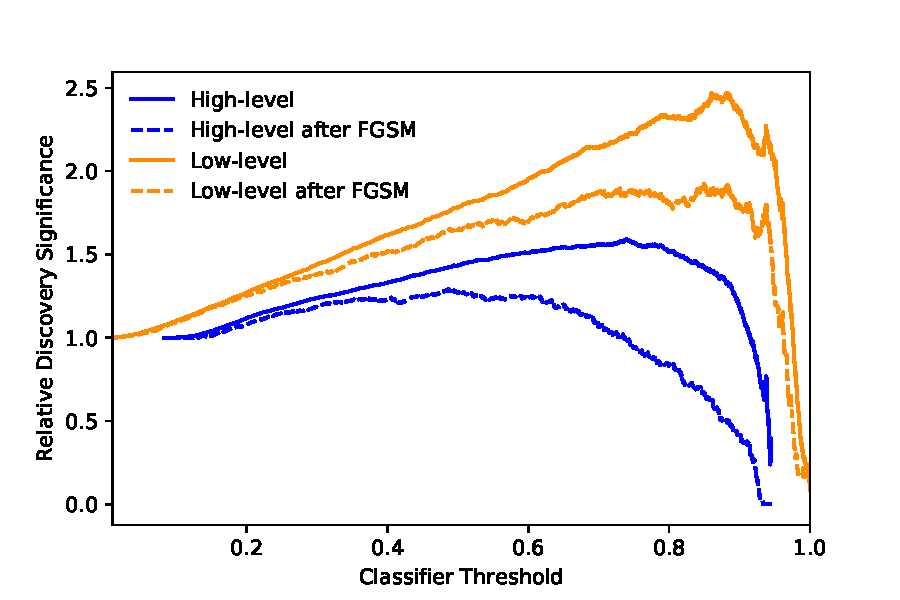
\includegraphics[width=0.45\textwidth]{figures/FGSM_Significance.pdf}\\
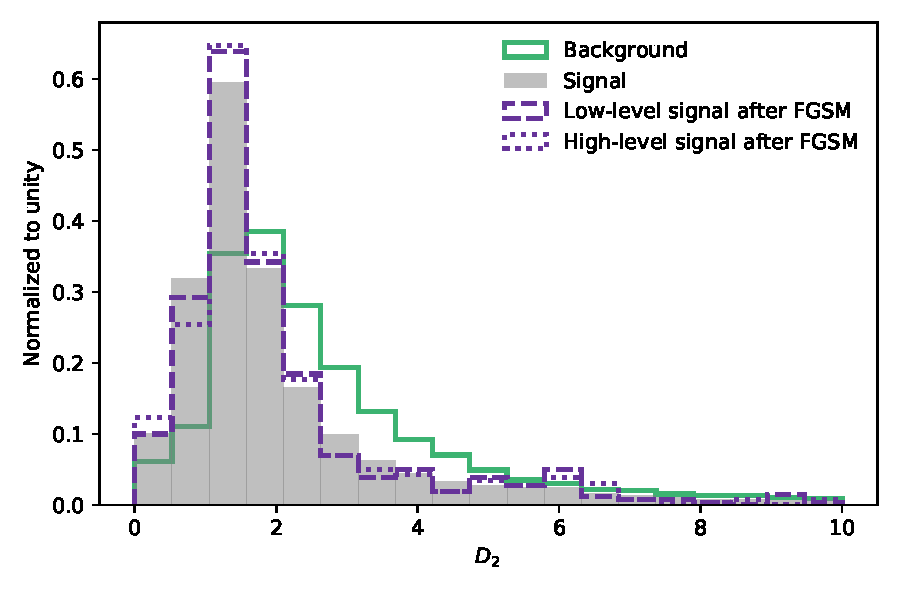
\includegraphics[width=0.4\textwidth]{figures/FGSM_D2.pdf}
\caption{Top: The relative discovery significance (true positive rate / square root of false positive rate) as a function of the classifier threshold for HL observables and LL observables before and after the FGSM attack described in Sec.~\ref{subsec:fgsm}.  Bottom: the $D_2$ observable before and after the FGSM attack for signal and background. }
\label{fig:FGSM2}
\end{figure}

While the FGSM illustrated the sensitivity to small perturbations for single jets, it does not show how systematic ensemble perturbations could modify the classifier performance.  Figure~\ref{fig:method2} is the result of an attack by an adversarial neural network.  Describe the figure. 

\begin{figure}[h!]
\centering
%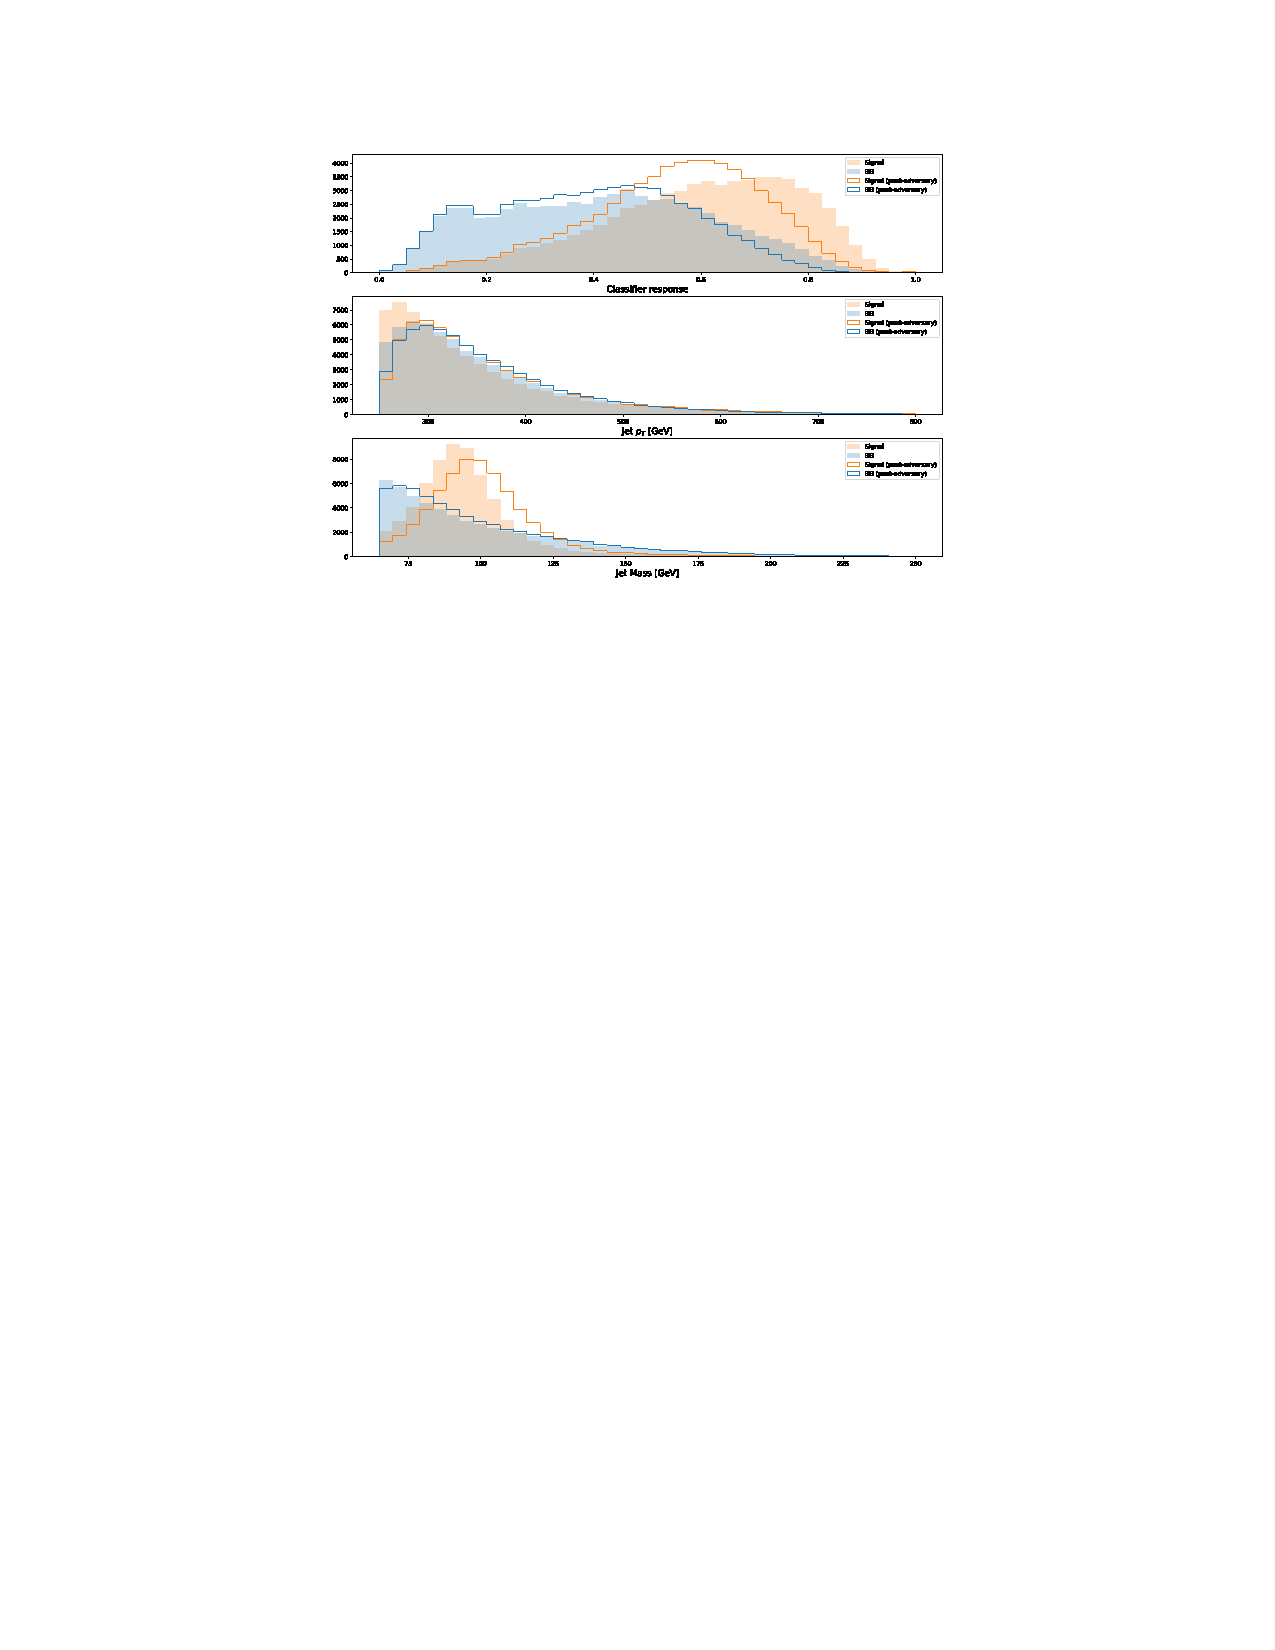
\includegraphics[width=0.45\textwidth]{figures/MethodBFig2.pdf}
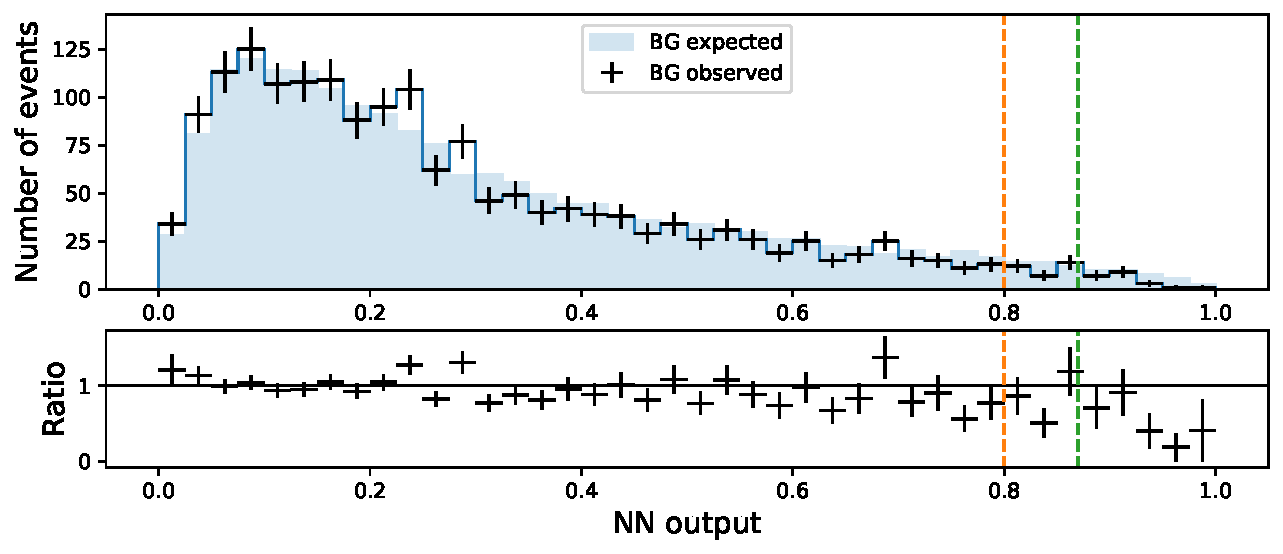
\includegraphics[width=0.45\textwidth]{figures/pseudodata_NN_PFN.pdf} \\
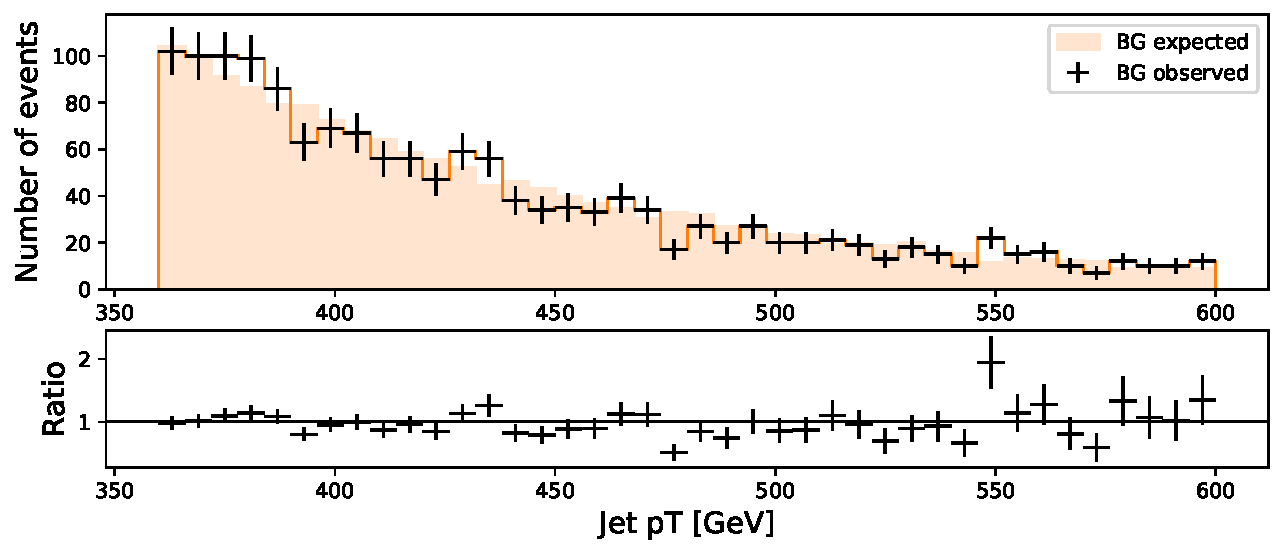
\includegraphics[width=0.45\textwidth]{figures/pseudodata_pt_PFN.pdf} \\
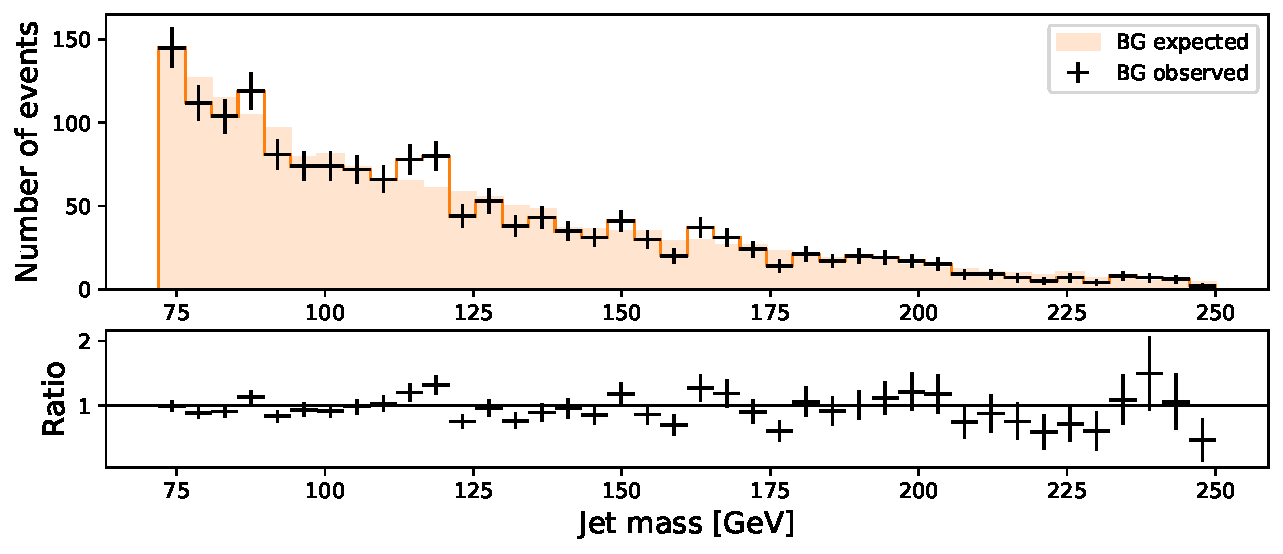
\includegraphics[width=0.45\textwidth]{figures/pseudodata_mass_PFN.pdf} 
\caption{Illustration of the effect of the adversarially-derived mismodelling for the low-level network.
Events to the left of the oragnge dashed line are in the control region.
Pseudodata (black points) are sampled from the BG distribution, with the adversarial perturbation applied; solid histograms show the unperturbed BG model.
(Top) The region to the left of the orange dashed line is the validation region, while events to the right of the green line are in the signal region.
(Middle, Bottom) The jet $\pt$ and mass distributions for events in the validation region.
Good agreement between pseudodata and the background model is observed in the validation region.
}
\label{fig:method2}
\end{figure}

The impact of the adversarial attack is quantified in Fig.~\ref{fig:method2b}.  Describe the figure. 

\begin{figure}[h!]
\centering
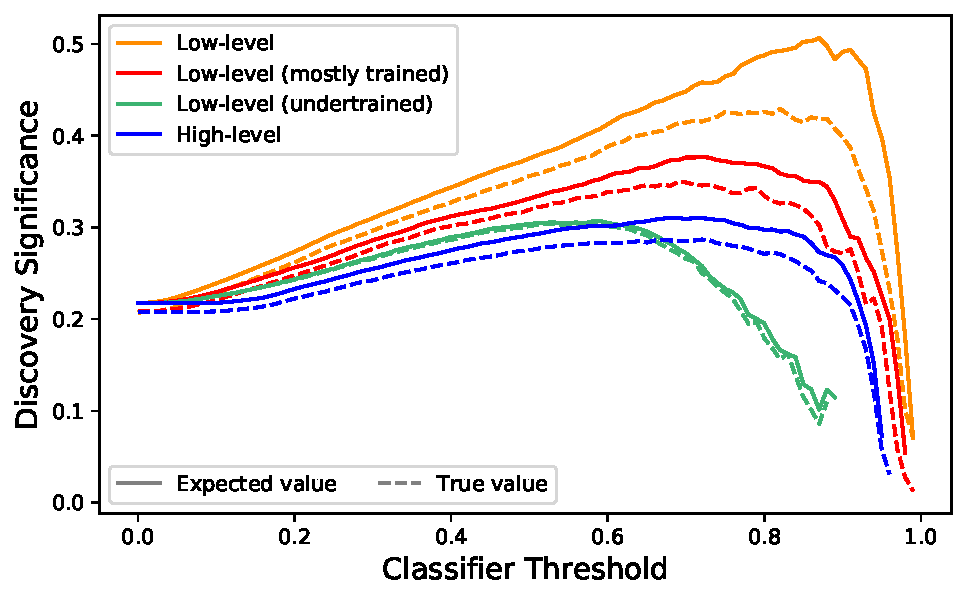
\includegraphics[width=0.45\textwidth]{figures/adversary_significance.pdf}
\caption{Effect of adversarial mismodelling on discovery significance, for high-level and low-level feature networks.
While the fully-trained low-level network is expected to perform better than the high-level network, it is also more strongly affected by an adversarial attack.
However, when deliberately undertrained, the low-level network is intentionally undertrained, its susceptibility is reduced.
}
\label{fig:method2b}
\end{figure}

\begin{figure}[h!]
\centering
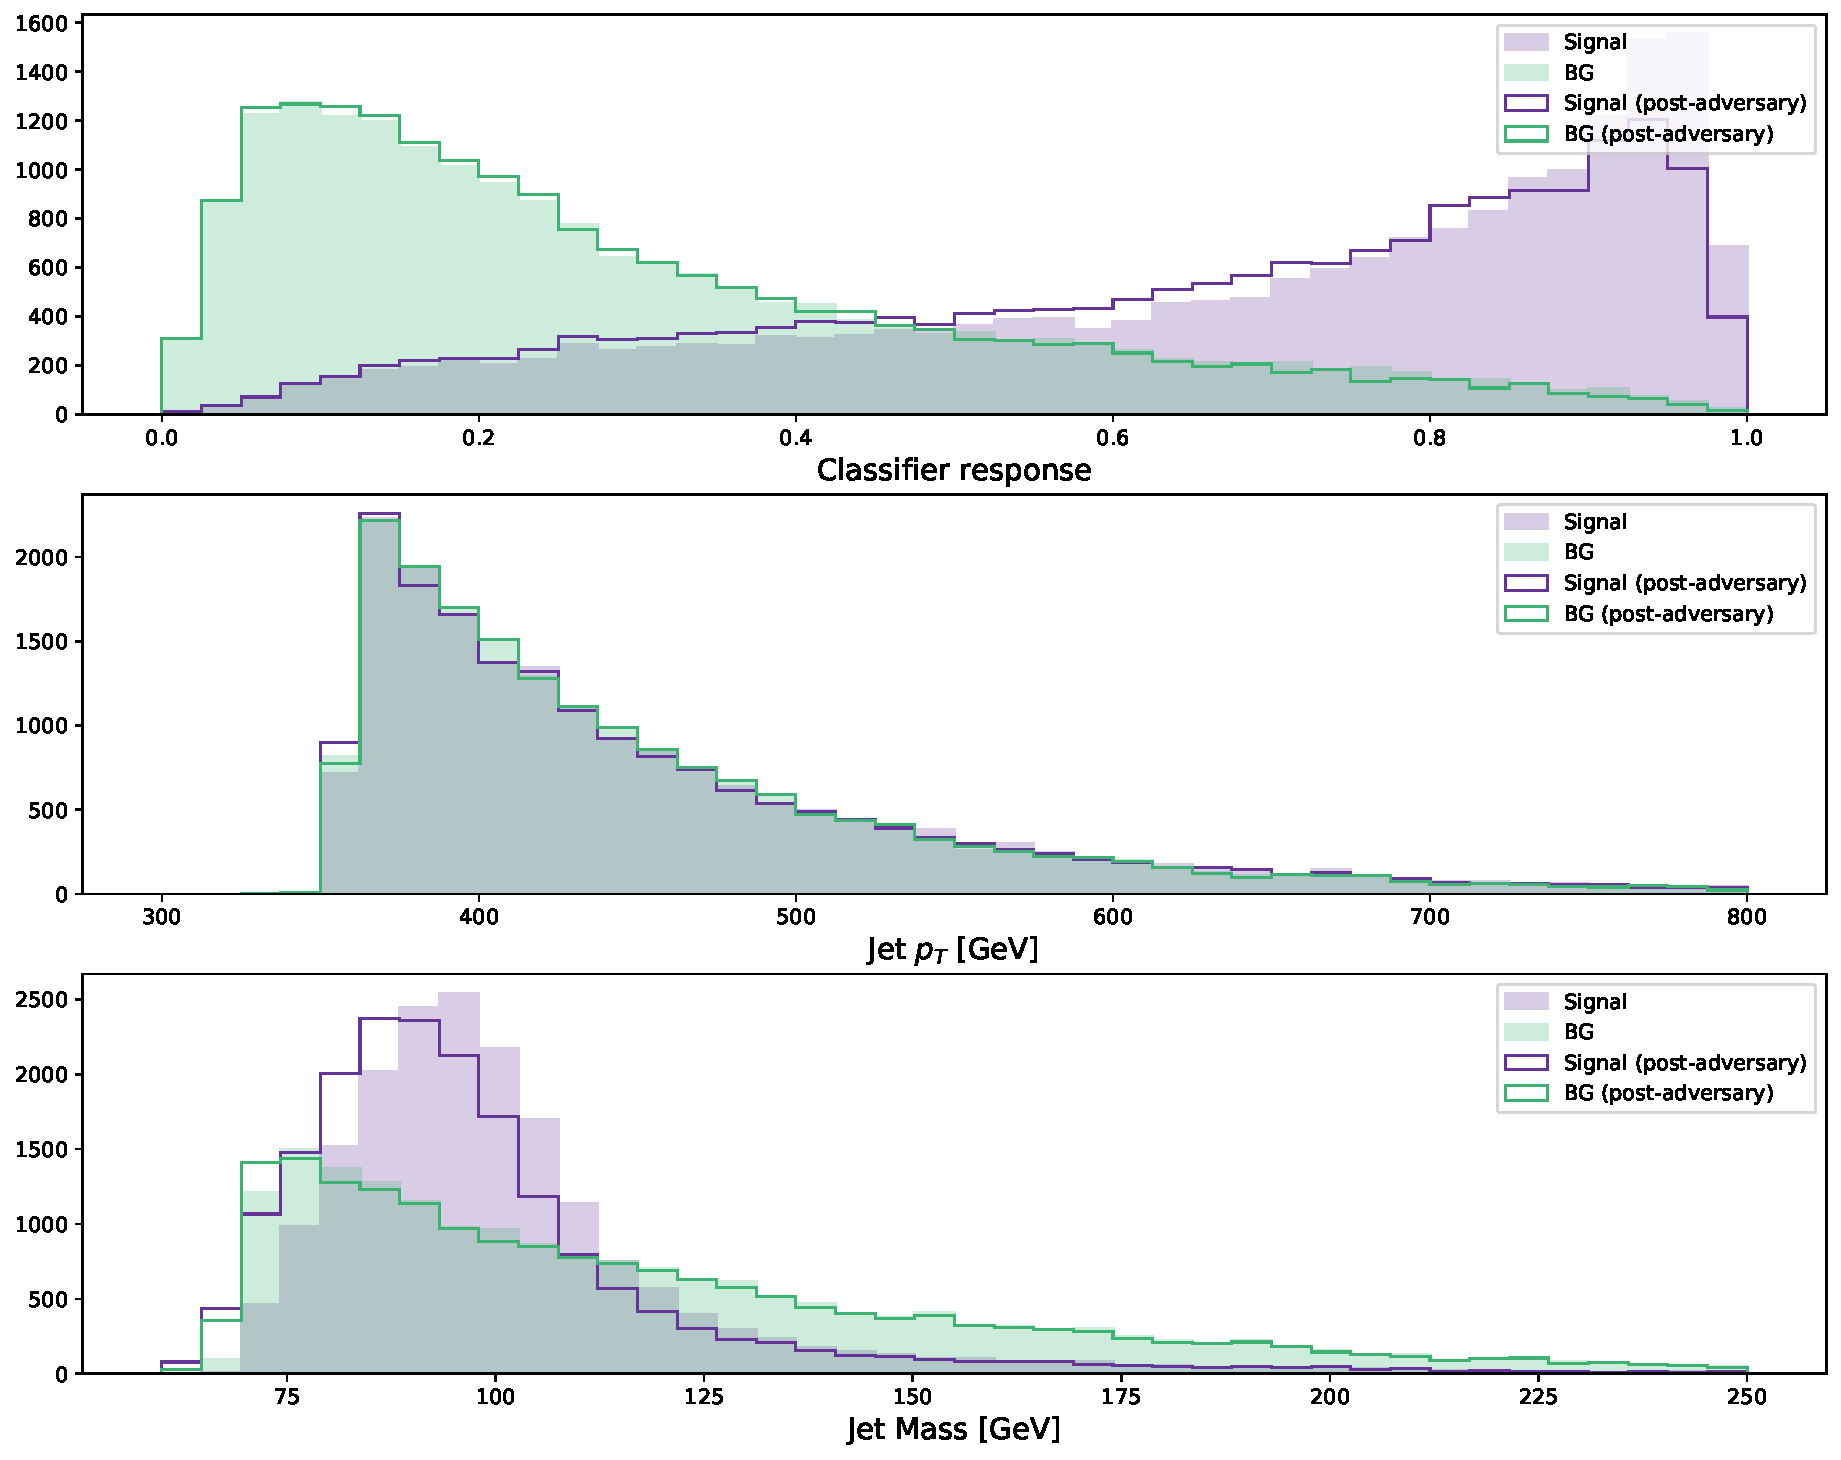
\includegraphics[width=0.45\textwidth]{figures/adv_classifer_response.pdf}
\caption{
Comparison of the adversary's effect on signal and background distributions for the low-level network.
}
\end{figure}

\begin{figure}[h!]
\centering
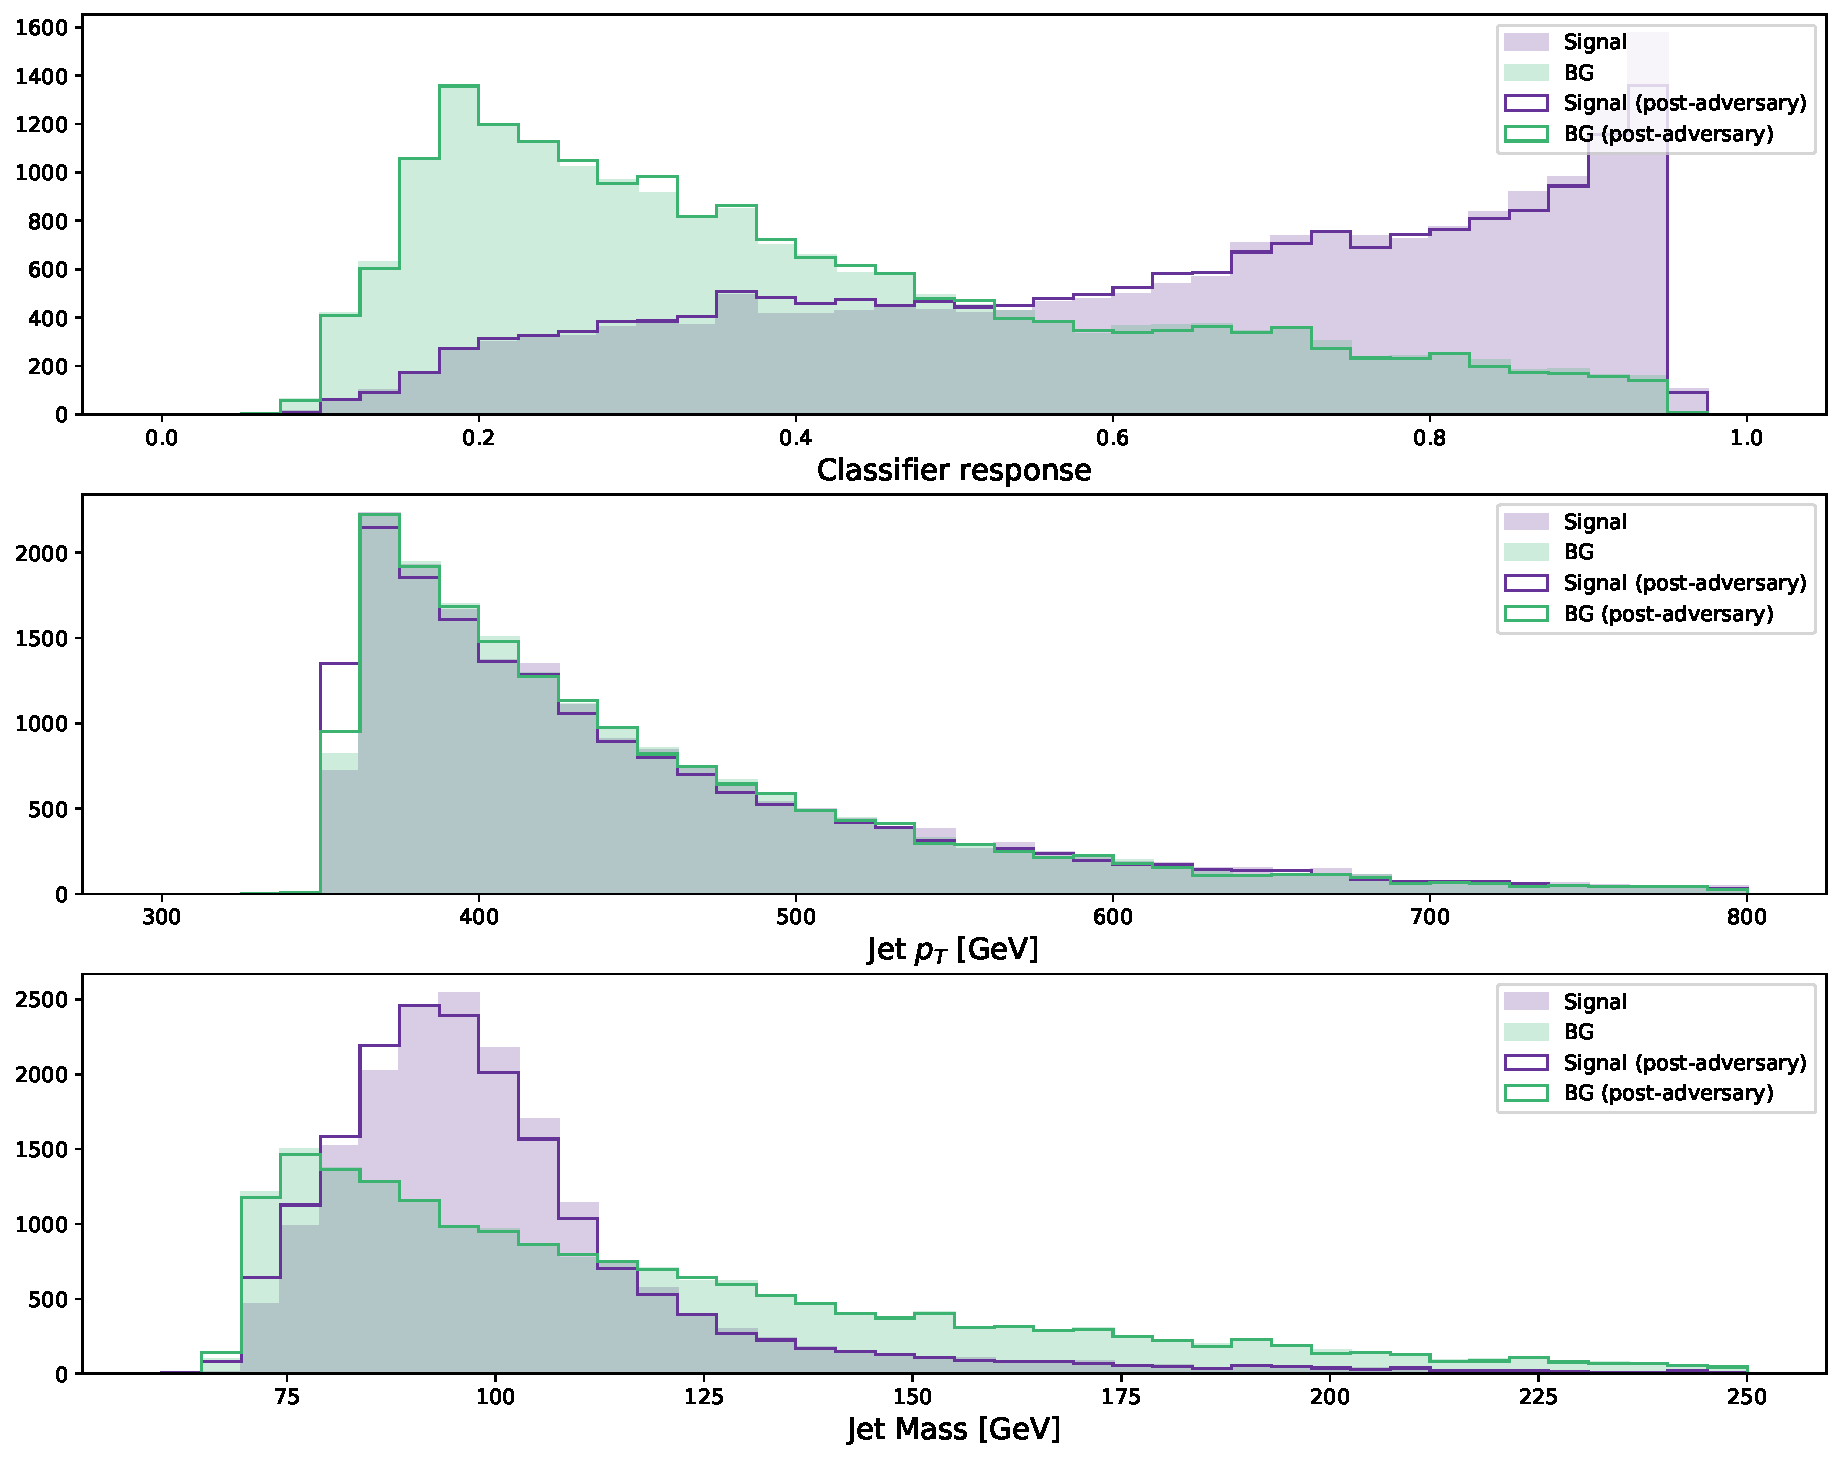
\includegraphics[width=0.45\textwidth]{figures/adv_classifer_response_HL.pdf}
\caption{
Comparison of the adversary's effect on signal and background distributions for the high-level network.
}
\end{figure}

%In general, high-dimensional inputs are quite susceptible to attack on the individual jet constituents, even at levels of perturbation which are small compared to detector resolution. However, is also important to consider the effect such attacks have on the observable physical quantities which are in practice validated by physicists. To this end, we introduce additional regularizing constraints on the attack by requiring the adversarially-perturbed event data leave various high-level observables, such as jet mass, in tact.

\clearpage

\section{Conclusions}

The interest in deep learning methods for HEP has grown significantly since the first studies were published five years ago~\cite{Baldi:2014kfa}.  While these methods hold great promise to enhance our sensitivity to discover new fundamental properties of nature, the traditional analysis techniques must be adapted.  We have shown that neural networks using high-dimensional low-level features are highly sensitive to mis-modeled inputs.  Current uncertainty estimates may not be accurate for high-dimensional features and traditional validation methods may not be able to detect such perturbations.  We have proposed adversarial approaches to bound the sensitivity of a deep learning-based analysis procedure.  While this is a crude bound, it may be used to establish robustness or diagnose situations where further studies are needed.  This work will hopefully begin a dialogue within the community about the robust application of deep learning to experimental measurements and searches.

\section*{ACKNOWLEDGMENTS}

This work is supported by the DOE under contract DE-AC02-05CH11231. 

\bibliography{myrefs}

\end{document}